\section{Algorithm Specification}

\subsection*{\textit{Version 1.0}}

\subsection{Introduction}

The CIShell Platform has been specifically designed around the idea of the
algorithm. It is the central and most important concept. Algorithms are fully
defined and self-contained bits of execution. They can do many things from data
conversion, data analysis, and can even spawn whole outside programs if needed.
Algorithms are very well defined black boxes in that what can come into and out
of the algorithm is specified in each algorithm's metadata. Other than that,
CIShell makes no attempt to understand the algorithm.

To be recognized by CIShell, an \class{AlgorithmFactory} must be registered with
OSGi's Service Registry. The service registry requires three things when
registering: an interface (\class{AlgorithmFactory}), an implementation, and a
\class{Dictionary} of metadata. The algorithm developer provides the
implementation and metadata. The metadata helps to differentiate and define the
algorithm for search and discovery, see section \ref{algMetaData}.

An algorithm defines its inputs in two ways. First, the input data is defined in
the algorithm's service metadata. Second, the acceptable user-entered parameters
are defined in a \class{MetaTypeProvider}, see section \ref{GUISpec}.

Figure \ref{fig:algExecWorkflow} shows the typical flow of information into and
out of an algorithm. First the input parameter specification is pulled from the
\class{AlgorithmFactory}. If parameters are needed, then a UI is created and user
inputs are entered. To create an \class{Algorithm}, the \class{AlgorithmFactory}
is passed the user-entered parameters, zero or more pieces of data, and a
\class{CIShellContext}. The \class{Algorithm} is then executed and produces zero
or more pieces of data.

\begin{figure}[htb!]
\centering
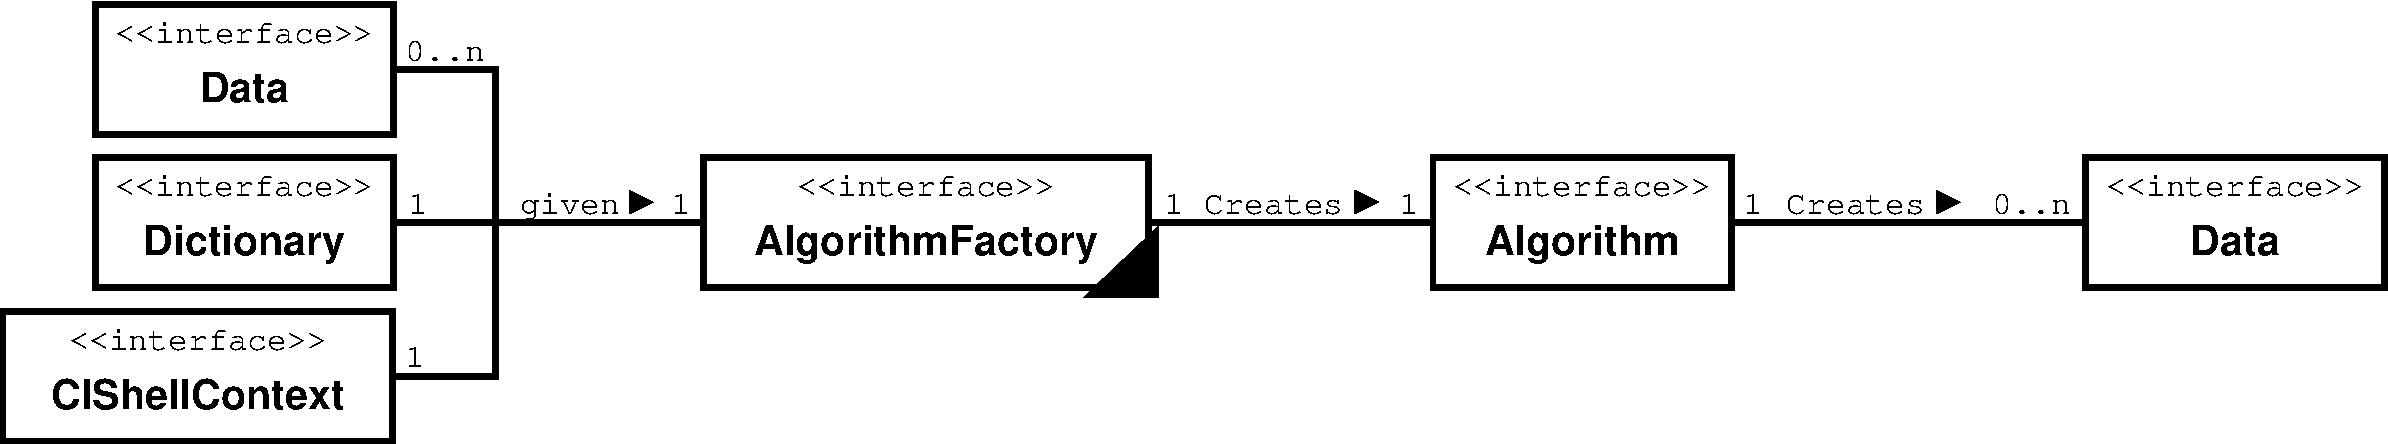
\includegraphics[width=150mm]{../img/algExecWorkflow.pdf}
\caption{Algorithm Execution Workflow}
\label{fig:algExecWorkflow}
\end{figure}

\subsection{Optional Interfaces}

Algorithm developers may augment algorithms with additional interfaces to enhance
parts of the execution workflow. An \class{AlgorithmFactory} can also implement
the \class{DataValidator} interface to validate the data beyond the data format
validation that an application should provide ahead of time. An \class{Algorithm}
can implement \class{ProgressTrackable} to allow for more detailed monitoring and
control of an \class{Algorithm}'s progress while executing. See each interface's
documentation for more details.

\subsection{Algorithm Service Metadata Definition}
\label{algMetaData}

When an algorithm is registered with OSGi's service registry, a dictionary of
metadata is provided. Since the algorithm itself is a black box, the metadata is
used to provide information about the algorithm. Information such as the format
of each \class{Data} item to be input and output is provided. In addition to the
mechanics of the algorithms, data such as the authors, label, urls, citation
references, and description are provided. This metadata can be searched by anyone
using OSGi's service registry to find relevant algorithms.

Each standard metadata element required by the CIShell specification is defined
below and in the interface \class{AlgorithmProperty}. It defines each key string
and the valid value strings to set in the metadata \class{Dictionary} when
registering an algorithm as a service.

\subsection*{service.pid}
A string that uniquely identifies the algorithm. The service.pid should not
change between sessions and only one algorithm with a given service.pid should
be available in the service registry at any given time. It is recommended to 
use the Java naming scheme including path for this purpose, i.e.,
``org.cishell.my.algorithm.MyAlgorithm''. This metadata element is defined
as part of the OSGi Service Platform Core Specification, section 6.1.12.58. 

\begin{quote}
\begin{description}
  \item[Example 1:] service.pid = org.cishell.my.algorithm.MyAlgorithm
\end{description}
\end{quote}

\subsection*{in\_data} Specifies the type and number of \class{Data} inputs the
algorithm accepts. The string is a comma separated list of data formats. There
are several valid strings for each data format. If a Java \class{Object} is
expected, use the expected full Java class as a string. If a \class{java.io.File}
is expected, use a string with the format ``file:\textit{mime/type}''. If a
\class{java.io.File} known only by file extension is expected (only applicable
for validator algorithms), a string with the format
``file-ext:\textit{file-extension}''. If no \class{Data} inputs are necessary
then the string ``null'' or not specifying the in\_data attribute at all is
valid. See section \ref{dataSpec} for more information on data format formatting.

\begin{quote}
\begin{description}
  \item[Example 1:] in\_data = null
  \item[Example 2:] in\_data = java.lang.String
  \item[Example 3:] in\_data = java.lang.String, file:text/plain, file:text/xml
  \item[Example 4:] in\_data = file-ext:xml
\end{description}
\end{quote}


\subsection*{out\_data} 
Specifies the type and number of \class{Data} outputs the
algorithm will produce when successfully run. This metadata key has the same
string format as defined in the in\_data specification. If no \class{Data}
outputs are produced then the string ``null'' or not specifying the out\_data
attribute at all is valid.

\begin{quote}
\begin{description}
  \item[Example 1:] out\_data = null
  \item[Example 2:] out\_data = java.lang.String
  \item[Example 3:] out\_data = java.lang.String, file:text/plain, file:text/xml
  \item[Example 4:] out\_data = file-ext:csv
\end{description}
\end{quote}

\subsection*{parentage}
If this metadata element is used, it defines how the output \class{Data}
produced by the algorithm should be arranged. \class{Data} items can be given a parent as
part of their metadata (which usually means the \class{Data} was derived from
the referenced \class{Data}). If parentage is set to ``default'' then each of the
algorithm's outputted \class{Data} items will have their parent \class{Data} item
set as the first inputted \class{Data} item (if applicable) by the
CIShell-conforming application. If parentage is set to something else or is not
set at all, then it is up to the algorithm to set up these relationships.

\begin{quote}
\begin{description}
  \item[Example 1:] parentage = default 
\end{description}
\end{quote}


\subsection*{type} 
Specifies the type of the algorithm. If no type is set, then
it is assumed to be of ``Standard Algorithm'' type. Which metadata keys to use
and their exact meaning varies depending on the type of algorithm. The different
algorithm types and their constraints are defined in section
\ref{algConstraints}.

\begin{quote}
\begin{description}
  \item[Example 1:] type = converter
  \item[Example 2:] type = validator
  \item[Example 3:] type = dataset 
\end{description}
\end{quote}


\subsection*{remotable}
Specifies if the algorithm can be run remotely. An algorithm can be run
remotely if it only uses the services provided by the \class{CIShellContext}
and does not create its own non-\class{GUIBuilderService}-built GUI. Valid
strings are ``true'' or ``false''. If this metadata element is not set, then
it is assumed that it cannot be run remotely.

\begin{quote}
\begin{description}
  \item[Example 1:] remoteable = true 
\end{description}
\end{quote}


\subsection*{label}
Specifies a human-readable short name for the algorithm. What label is
acceptable varies depending on the type of the algorithm. 

\begin{quote}
\begin{description}
  \item[Example 1:] label = Load\ldots 
\end{description}
\end{quote}


\subsection*{description}
Provides more details on the workings of the algorithm. What
description is acceptable varies depending on the type of the algorithm.

\begin{quote}
\begin{description}
  \item[Example 1:] description = Loads selected data into the data manager. 
\end{description}
\end{quote}


\subsection*{menu\_path}
Specifies where on the menu an algorithm is to be
placed if a menu bar is used. Otherwise, it can act as a primitive hierarchical
classification of the algorithm. The string is a ``/'' separated list with
each element in the list getting more specific. The last element in the list
specifies a group for grouping algorithms in its final menu. Possible groups
include: ``additions'' for default placement, ``start'' for being placed at
the start of the menu, or ``end'' for being placed at the end of the menu.

\begin{quote}
\begin{description}
  \item[Example 1:] menu\_path = File/additions
  \item[Example 2:] menu\_path = Analysis/Undirected Networks/start
  \item[Example 3:] menu\_path = Visualization/Networks/end
\end{description}
\end{quote}


\subsection*{conversion}
For converter algorithms, this metadata element specifies if any data is
lost in the conversion. Possible values are ``lossy'' and ``lossless''. A
description of what type of information is lost should be explained in the
description.

\begin{quote}
\begin{description}
  \item[Example 1:] conversion = lossy 
\end{description}
\end{quote}


\subsection*{authors}
A comma separated list of the authors of the abstract algorithm.

\begin{quote}
\begin{description}
  \item[Example 1:] authors = Bruce Herr
  \item[Example 2:] authors = Bruce Herr, Weixia Huang, Katy Borner 
\end{description}
\end{quote}


\subsection*{implementers}
A comma separated list of the developers who implemented the algorithm in code.

\begin{quote}
\begin{description}
  \item[Example 1:] implementers = Bruce Herr
  \item[Example 2:] implementers = Bruce Herr, Weixia Huang, Katy Borner 
\end{description}
\end{quote}


\subsection*{integrators}
A comma separated list of the developers who integrated the algorithm code as
a compliant cishell algorithm.

\begin{quote}
\begin{description}
  \item[Example 1:] integrators = Bruce Herr
  \item[Example 2:] integrators = Bruce Herr, Weixia Huang, Katy Borner 
\end{description}
\end{quote}


\subsection*{documentation\_url}
A URL to relevant documentation for the algorithm.

\begin{quote}
\begin{description}
  \item[Example 1:] documentation\_url = http://cishell.org/dev/ 
\end{description}
\end{quote}


\subsection*{reference}
A formal reference to a paper explaining the abstract algorithm.

\begin{quote}
\begin{description}
  \item[Example 1:] reference = Herr, Bruce W., Huang, Weixia, Penumarthy,
  Shashikant, Börner, Katy. (2007) Designing Highly Flexible and Usable 
  Cyberinfrastructures for Convergence. In William S. Bainbridge and Mihail C. 
  Roco (Eds.) Progress in Convergence – Technologies for Human Wellbeing. 
  Annals of the New York Academy of Sciences, Boston, MA, volume 1093, pp. 161-179.
\end{description}
\end{quote}


\subsection*{reference\_url}
A URL to a paper explaining the abstract algorithm.

\begin{quote}
\begin{description}
  \item[Example 1:] reference\_url = http://cishell.org/papers/06-cishell.pdf 
\end{description}
\end{quote}


\subsection*{written\_in}
A comma separated list of the programming languages used to implement and
integrate the algorithm code.

\begin{quote}
\begin{description}
  \item[Example 1:] written\_in = Java
  \item[Example 2:] written\_in = Java, C++ 
\end{description}
\end{quote}
